\documentclass[12pt]{article}
\usepackage{geometry}
\geometry{a4paper, portrait, margin=1in}

% --- Math Packages ---
\usepackage{amsmath}
\usepackage{amssymb}
\usepackage{amsfonts}
\usepackage{amsthm}

% --- Graphics & Diagrams ---
\usepackage{graphicx}
\usepackage{tikz}
\usetikzlibrary{shapes, arrows, positioning}

% --- Formatting ---
\usepackage{parskip}
\usepackage[hidelinks]{hyperref}
\usepackage{natbib}
\usepackage{enumitem}

\pagestyle{plain}

\title{Initial Model}
\author{Mohammad-Shah Karim}
\date{February 2026}

\begin{document}

\maketitle

\tableofcontents

\newpage

\section{Introduction}

This document outlines a game-theoretical model for pharmaceutical innovation and pricing to explain the empirical puzzle observed in the patent market following the expansion of Medicaid under the Affordable Care Act. The model captures the stochastic nature of R\&D and the specific procurement mechanism (PDL bidding) used by state agencies.

Figure \ref{fig:game_structure} summarises the sequence of play, mapping the innovation decision in Stage 1 to the pricing outcomes in Stage 3.

\begin{figure}[h]
    \centering
    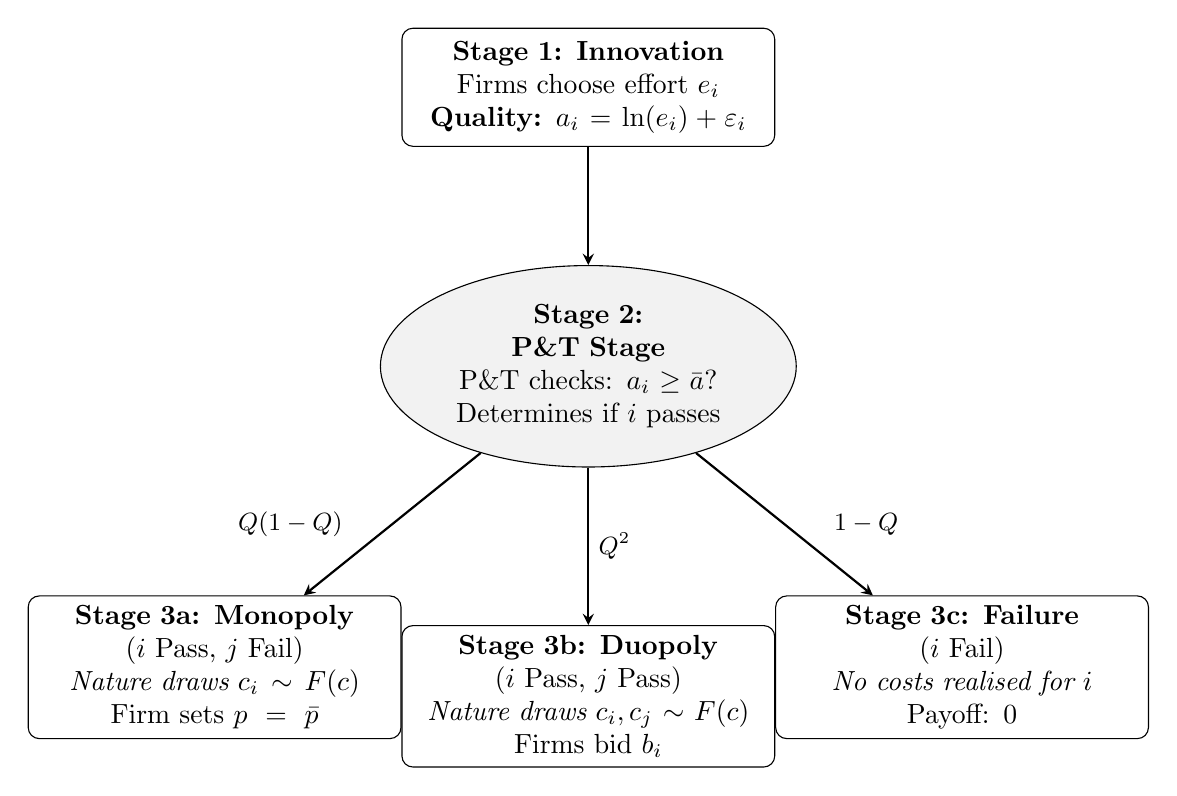
\begin{tikzpicture}[
        node distance=1.5cm and 1cm,
        auto,
        block/.style={rectangle, draw, fill=white, text width=4.5cm, align=center, rounded corners, minimum height=1.5cm},
        cloud/.style={ellipse, draw, fill=gray!10, text width=3.5cm, align=center, minimum height=1.2cm},
        arrow/.style={thick,->,>=stealth}
    ]

    % Stage 1: Innovation
    \node [block] (stage1) {\textbf{Stage 1: Innovation}\\ Firms choose effort $e_i$\\ \textbf{Quality:} $a_i = \ln(e_i) + \varepsilon_i$};

    % Stage 2: P&T Stage
    \node [cloud, below=of stage1] (pt) {\textbf{Stage 2: P\&T Stage}\\ P\&T checks: $a_i \ge \bar{a}$?\\ Determines if $i$ passes};
    
    % Stage 3: Pricing & Costs
    % Monopoly
    \node [block, below left=2cm and 0.5cm of pt] (mono) {\textbf{Stage 3a: Monopoly}\\ ($i$ Pass, $j$ Fail)\\ \textit{Nature draws $c_i \sim F(c)$}\\ Firm sets $p = \bar{p}$};
    
    % Duopoly
    \node [block, below=2cm of pt] (duo) {\textbf{Stage 3b: Duopoly}\\ ($i$ Pass, $j$ Pass)\\ \textit{Nature draws $c_i, c_j \sim F(c)$}\\ Firms bid $b_i$};
    
    % Failure
    \node [block, below right=2cm and 0.5cm of pt] (fail) {\textbf{Stage 3c: Failure}\\ ($i$ Fail)\\ \textit{No costs realised for $i$}\\ Payoff: 0};

    % Connecting Lines
    \draw [arrow] (stage1) -- (pt);
    \draw [arrow] (pt) -- node[left, xshift=-0.5cm, font=\small] {$Q(1-Q)$} (mono);
    \draw [arrow] (pt) -- node[font=\small] {$Q^2$} (duo);
    \draw [arrow] (pt) -- node[right, xshift=0.5cm, font=\small] {$1-Q$} (fail);

    \end{tikzpicture}
    \caption{The Sequence of Play: Innovation, P\&T Approval, and Pricing}
    \label{fig:game_structure}
\end{figure}

\newpage

\section{Stage 1: The Innovation Decision (Effort)}

First, firms make investment decisions for a drug they wish to market. Innovation is modelled to require effort - this is costly but improves the probability of clinical success.

\subsection{The Production Technology}
The realised clinical quality $a_i$ is a function of the effort exerted by the firm and a stochastic component $\varepsilon_i$:
\begin{equation}
    a_i = \ln(e_i) + \varepsilon_i, \qquad \varepsilon_i \sim N(0, \sigma^2)
\end{equation}
where $\varepsilon_i$ represents the inherent uncertainty of the R\&D process.

\subsection{The Cost of Effort}
Firms $i$ and $j$ simultaneously choose R\&D effort levels $e_i \geq 0$. Effort is assumed to be costly and convex:
\begin{equation}
    C(e_i) = \frac{1}{2} k e_i^2
\end{equation}

\newpage

\section{Stage 2: The P\&T Stage}
Once effort is exerted it is now a sunk cost, nature determines the clinical outcome of each firm's drug $a_i$, i.e. whether the drug passes the P\&T stage.

\subsection{The Approval Condition}
A drug is clinically approved (passes the P\&T stage) if its quality $a_i$ exceeds a regulatory threshold $\bar{a}$:

\begin{equation}
    \text{P\&T Stage}_i = 
    \begin{cases} 
        \text{Approved} & \text{if } a_i \geq \bar{a} \\
        \text{Not Approved} & \text{if } a_i < \bar{a}
    \end{cases}
\end{equation}

\subsection{The Probability of Success ($Q$)}
The probability of passing, denoted $Q(e_i)$, is endogenous to effort:

\begin{align}
    Q(e_i) &= \Pr(\ln e_i + \varepsilon_i \geq \bar{a}) \\
           &= \Pr(\varepsilon_i \geq \bar{a} - ln e_i) \\
           &= 1 - \Pr(\varepsilon_i \geq \bar{a} - ln e_i) \\
           &= 1 - \Phi\left(\frac{\bar{a} - \ln e_i}{\sigma}\right)
\end{align}

where $\Phi(\cdot)$ is the standard normal CDF. \vspace{1em}

This defines the transition probabilities into Stage 3.

\newpage

\section{Stage 3: The Pricing Subgame}
Firms that pass Stage 2 compete for market access. A rebate wedge $\tau(M)$ is introduced, where $\tau'(M) > 0$ - this represents the state's increasing monopsony power as their market size $M$ grows.

The game resolves into one of three mutually exclusive states.

\subsection{Stage 3a: The Monopoly State}

\textbf{Condition:} Firm $i$ passes while firm $j$ fails:
\begin{align*}
    a_i \geq \bar{a} > a_j
\end{align*}

\textbf{Mechanism:} Firm $i$ is the sole player in the market and negotiates directly with the state.

\paragraph{Setup} 
The firm faces a market demand $M$ which is perfectly inelastic with respect to price since Medicaid patients are fully insured under the programme. However, the state imposes a maximum allowable price $\bar{p}$ and the firm also pays some rebate $\tau(M)$.

\paragraph{Optimisation Problem}
The firm chooses price $p$ to maximise profit:
\begin{equation}
    \max_{p} \pi_i = M(p - c_i - \tau(M)) \quad \text{s.t.} \quad p \le \bar{p}
\end{equation}
Since demand is inelastic, the profit function is strictly increasing in $p$.

\paragraph{Equilibrium Result}
The firm sets the price at the binding cap: $p^* = \bar{p}$, and the resulting profit is:
\begin{equation} \label{eq:mono_profit}
    \pi_i^{Mono}(c_i) = M(\bar{p} - c_i - \tau(M))
\end{equation}
Denote the expected value of this state across marginal costs as: 

\begin{equation}
V^M = \mathbb{E}_c[\pi_i^{Mono}]
\end{equation}

\subsection{Stage 3b: The Duopoly State (Auction)}
\textbf{Condition:} Both firms pass the P\&T stage:

\begin{align*}
    a_i \geq \bar{a}, \qquad a_j \geq \bar{a}
\end{align*}

\textbf{Mechanism:} Firms compete in a first-price sealed-bid procurement auction.

\paragraph{Setup}
Each firm independently draws a marginal cost $c_i, c_j$ from a common distribution $F(c)$ with support $[\underline{c}, \bar{c}]$. Each firm submits a sealed bid (net price) $b_i$. The lowest bidder wins PDL status and obtains the full market volume $M$ minus the statutory wedge.
\[
\pi_i =
\begin{cases}
M\big(b_i - c_i - \tau(M)\big) & \text{if } b_i \leq b_j, \\
0 & \text{if } b_i > b_j.
\end{cases}
\]

\paragraph{Equilibrium Derivation}
Assume that there exists a strictly increasing and differentiable symmetric Bayesian-Nash Equilibrium bidding strategy $b(c)$.

\subparagraph{Step 1: The Probability of Winning}
Suppose firm $i$ has cost $c$ but considers submitting a bid $\tilde{b}$ corresponding to the optimal bid of type $t$ (i.e., $\tilde{b} = b(t)$). Firm $i$ wins if its bid is lower than the rival's bid $b(c_j)$:
\begin{equation}
    b(t) < b(c_j) \iff t < c_j
\end{equation}
The probability of winning is therefore:
\begin{equation}
    \Pr(\text{win}) = \Pr(c_j > t) = 1 - F(t)
\end{equation}

\subparagraph{Step 2: The Optimisation Problem}
The firm chooses the target type $t$ to maximise expected profit. Let $\tilde{c} = c + \tau(M)$ denote the effective cost including the statutory wedge.
\begin{equation}
    \max_{t} \mathbb{E}[\pi(t, c)] = M(b(t) - c - \tau(M))[1 - F(t)]
\end{equation}
Let $U(c)$ be the value function (maximum expected profit) for a firm with true cost $c$:
\begin{equation}
    U(c) = \max_{t} M(b(t) - c - \tau(M))[1 - F(t)]
\end{equation}

\subparagraph{Step 3: Applying the Envelope Theorem}
Differentiation of the value function $U(c)$ with respect to cost $c$ yields the partial derivative of the objective function evaluated at the optimal choice $t=c$ (truth-telling):
\begin{equation}
    U'(c) = \left. \frac{\partial \mathbb{E}[\pi(t, c)]}{\partial c} \right|_{t=c} = -M[1 - F(c)]
\end{equation}

\subparagraph{Step 4: Solving for Expected Profit}
Integrating $U'(c)$ from $c$ to $\bar{c}$, and noting that profit at the highest cost type $U(\bar{c}) = 0$:
\begin{equation} \label{eq:value_integral}
    U(c) = M \int_{c}^{\bar{c}} (1 - F(u)) \, du
\end{equation}

\subparagraph{Step 5: Recovering the Bidding Function}
Equating the integral expression (\ref{eq:value_integral}) with the definition of profit at the optimum yields the symmetric equilibrium bidding strategy:
\begin{equation} \label{eq:bid_function}
    b(c) = c + \tau(M) + \frac{\int_{c}^{\bar{c}} (1 - F(u)) \, du}{1 - F(c)}
\end{equation}

\paragraph{Equilibrium Result (Expected Payoff)}
Substituting the optimal bid, the ex-ante expected profit for entering Stage 3b is:
\begin{equation} \label{eq:duo_profit}
    \Pi^{Duo}(c) = M \int_{c}^{\bar{c}} (1 - F(u)) \, du
\end{equation}

Denote the expected value of this state across marginal costs as: 

\begin{equation}
V^D = \mathbb{E}_c[\Pi^{Duo}]    
\end{equation}


\subsection{Stage 3c: The Failure State}
\textbf{Condition:} Firm $i$ fails:
\begin{align*}
    a_i < \bar{a}
\end{align*}

The firm fails to meet the clinical threshold required for PDL consideration. It cannot submit a bid.

\paragraph{Equilibrium Result}
The firm does not enter the market and earns zero revenue.
\begin{equation}
    \pi_i^{Fail} = 0
\end{equation}

\newpage

\section{Equilibrium Analysis}
Solve for the optimal effort $e^*$ by maximising the total expected profit across the three possible outcomes of Stage 3.

\subsection{The Maximisation Problem}
The firm chooses effort $e_i$ to maximise total expected profit. The objective function $\Psi_i$ is the probability-weighted sum of the payoffs in each state minus the cost of effort:

\begin{equation}
    \max_{e_i} \Psi_i = \underbrace{Q(e_i)[1-Q(e_j)] V^M}_{\text{Stage 3a Incentive}} + \underbrace{Q(e_i)Q(e_j) V^D}_{\text{Stage 3b Incentive}} - \frac{1}{2} k e_i^2
\end{equation}

where $V^M$ and $V^D$ are the expected values derived in the monopoly and duopoly cases respectively.

\subsection{Optimal Effort ($e^*$)}
The First Order Condition (FOC) with respect to effort $e_i$ is derived by differentiating $\Psi_i$:
\begin{equation}
    \frac{\partial \Psi_i}{\partial e_i} = Q'(e_i)(1-Q(e_j)) V^M + Q'(e_i)Q(e_j) V^D - k e_i = 0
\end{equation}
This yields the following expression, where the margin benefit of effort is equal to the associated marginal cost:
\begin{equation} \label{eq:FOC_final}
    Q'(e_i) \left[ (1-Q(e_j)) V^M + Q(e_j) V^D \right] = k e_i
\end{equation}
The term in square brackets is the \textbf{Expected Prize}. In a symmetric equilibrium where $e_i = e_j = e^*$, this implicitly defines the optimal effort level $e^*$.

\subsection{The ``Incentive Trap'' Mechanism}
Now derive the effect of the expansion of Medicaid ($M \uparrow$) on innovation effort $e^*$. Innovation falls if the marginal benefit of effort decreases with market size.

\paragraph{The Mechanism}
\begin{enumerate}
    \item \textbf{Stage 3b (Duopoly) is Robust:} From Equation (\ref{eq:duo_profit}), $V^D$ scales linearly with $M$. Expansion increases the value of the competitive state.
    \item \textbf{Stage 3a (Monopoly) is Vulnerable:} From Equation (\ref{eq:mono_profit}), the value of the monopoly state is $V^M = M(\bar{p} - \bar{c} - \tau(M))$. The effect of expansion is unclear:
    \begin{equation}
        \frac{d V^M}{d M} = \underbrace{(\bar{p} - \bar{c} - \tau)}_{\text{Volume Effect (+) }} - \underbrace{M \tau'(M)}_{\text{Monopsony Effect (-) }}
    \end{equation}
\end{enumerate}

\paragraph{Conclusion}
If the elasticity of the rebate $\epsilon_{\tau, M}$ is sufficiently large, the monopsony effect dominates, resulting in the the value of Stage 3a (the monopoly) to collapse. Since the monopoly stage (3a) is the primary driver of R\&D investment ($V^M \gg V^D$), the total incentive to innovate falls, explaining the negative coefficient observed in the data.

\end{document}